\subsection{\textsf{FSM}: A \DSL for Finite-State Machines}
\label{sec:Examples:FSM}

Finite State Machines (FSM) represent a common \DSL for capturing state-based 
behaviour of various biological, but also computational domains (e.g. Turing 
Machines, but also Chomsky's Regular Grammars, among others). This Section considers
FSMs that are simplified in various ways: in particular, we only consider a
word acceptance semantics where transitions do not contain guards and triggers are
reduced to their simplest expression, namely simple strings.

\subsubsection{Specification}
\label{sec:Examples:FSM:Specification}

\begin{figure}%
   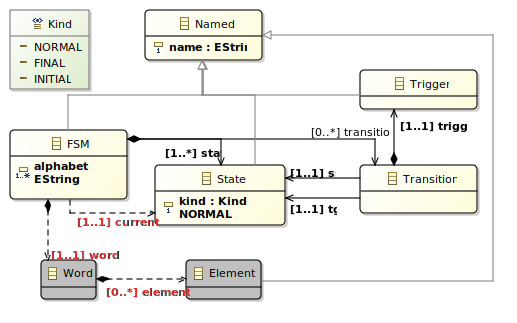
\includegraphics[width=\columnwidth]{FSM}%
   \caption{A metamodel for Finite State Machines.}%
   \label{fig:FSM_MM}%
\end{figure}


\autoref{fig:FSM_MM} (top) specifies the metamodel of the Finite State Machine \DSL. 
An \textsf{FSM} is composed of \textsf{State}s identified by a \textsf{name}, and
\textsf{Transition}s that contain a simple \textsf{Trigger}, specified as 
\textsf{name}d event. \autoref{fig:FSM_M} depicts a simple model consisting of 
three \textsf{State}s and three \textsf{Transition}s, to recognise the regular 
expression $\mathtt{(a\cdot b)^\star\ b}$. 

We assume the classical visual representation for \textsf{FSM}: a \textsf{State}
is represented by a circle labelled with its \textsf{name}; and a 
\textsf{Transition} is represented by an arrow pointing to its \textsf{tgt} and 
carrying the \textsf{Trigger}'s name as a label. We represent the \textsf{current}
\textsf{State} by surimposing a red rounded form (that we call \emph{token}) over
the corresponding \textsf{State} (cf. \autoref{fig:FSM_M}).


\subsubsection{Execution}
\label{sec:Examples:FSM:Execution}

We adopt a \emph{word-recognising} semantics encoded in a transformation called
\textsf{accept} that reads a \textsf{Word} and traverses the \textsf{FSM}. A 
\textsf{Word} is accepted iff the \textsf{current} \textsf{State} of the \textsf{FSM}
is \textsf{FINAL} when the \textsf{Word} becomes empty.

\subsubsection{Animations}
\label{sec:Examples:FSM:Animations}

Typically, \textsf{accept} is implemented using a sub-transformation 
\textsf{fire(e : Element) : State [0..1]} that determines which \textsf{State} 
to update to when consuming an \textsf{Element} \textsf{e}, making it a good 
candidate for four different animations, when \textsf{fire} returns an actual 
\textsf{State}:
\begin{description}
   \item[FSM.1] The token disappears from the \textsf{current} \textsf{State} and
   reappears inside the updated \textsf{current};
   \item[FSM.2] The token disappears from the \textsf{current} \textsf{State}, and
   slides along the entire arrow of the fired \textsf{Transition}, then appears in
   the updated \textsf{current};
   \item[FSM.3] The token disappears from the \textsf{current} \textsf{State}, the
   arrow of the fired \textsf{Transition} blinks in red for 2 seconds, then the 
   token reappears in the updated \textsf{current}.
\end{description}


\begin{figure}[t]%
   \centering
   \begin{subfigure}[b]{0.45\columnwidth}
      \centering
      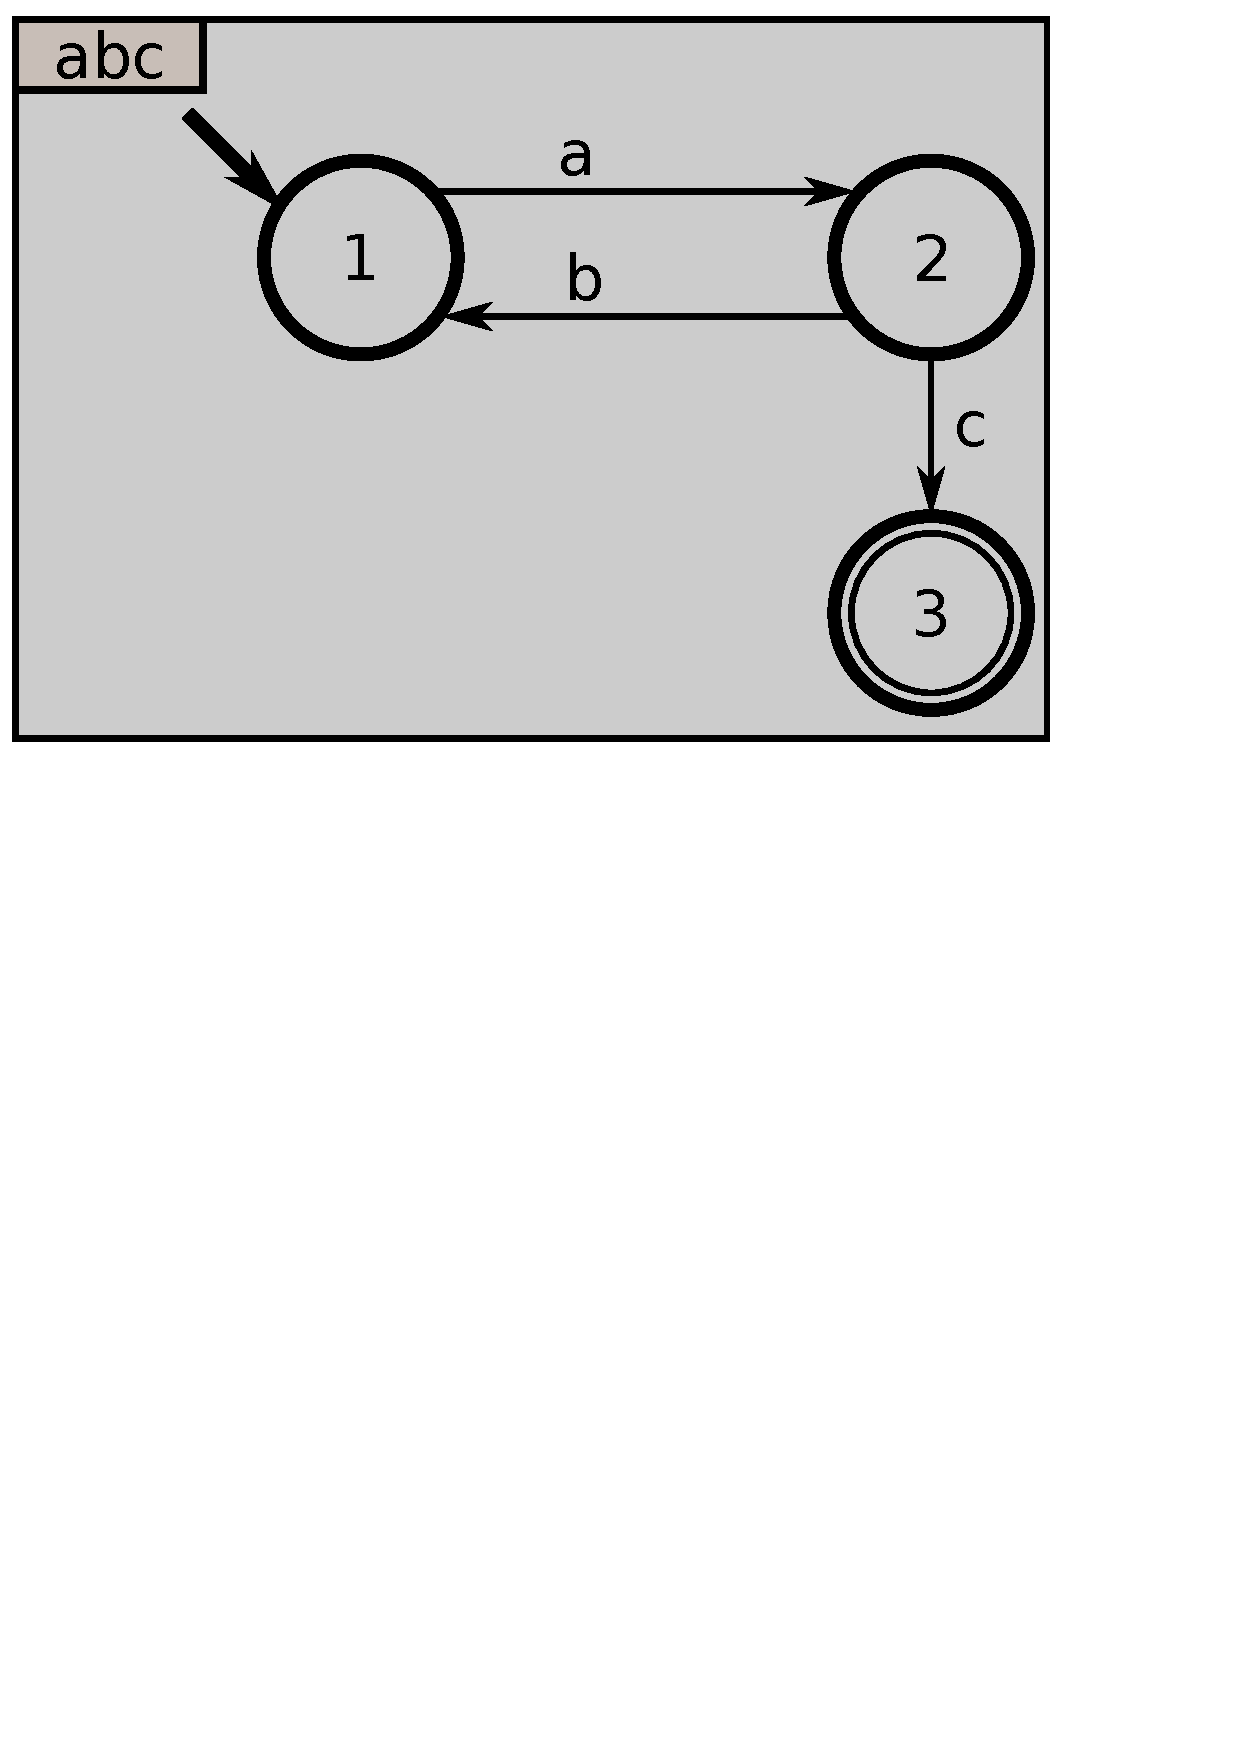
\includegraphics[width=\columnwidth, clip, trim=0cm 17cm 3cm 0cm]{FSM_M.pdf}%
      \caption{Editing \textsf{abc} to obtain a 3-state/3-transition FSM model: 
      states \textsf{1} and \textsf{3} are respectively \textsf{INITIAL} and 
      \textsf{FINAL}.}
      \label{fig:FSM:Model:Edition}
   \end{subfigure}
   \hfill
   \begin{subfigure}[b]{0.45\columnwidth}
      \centering
      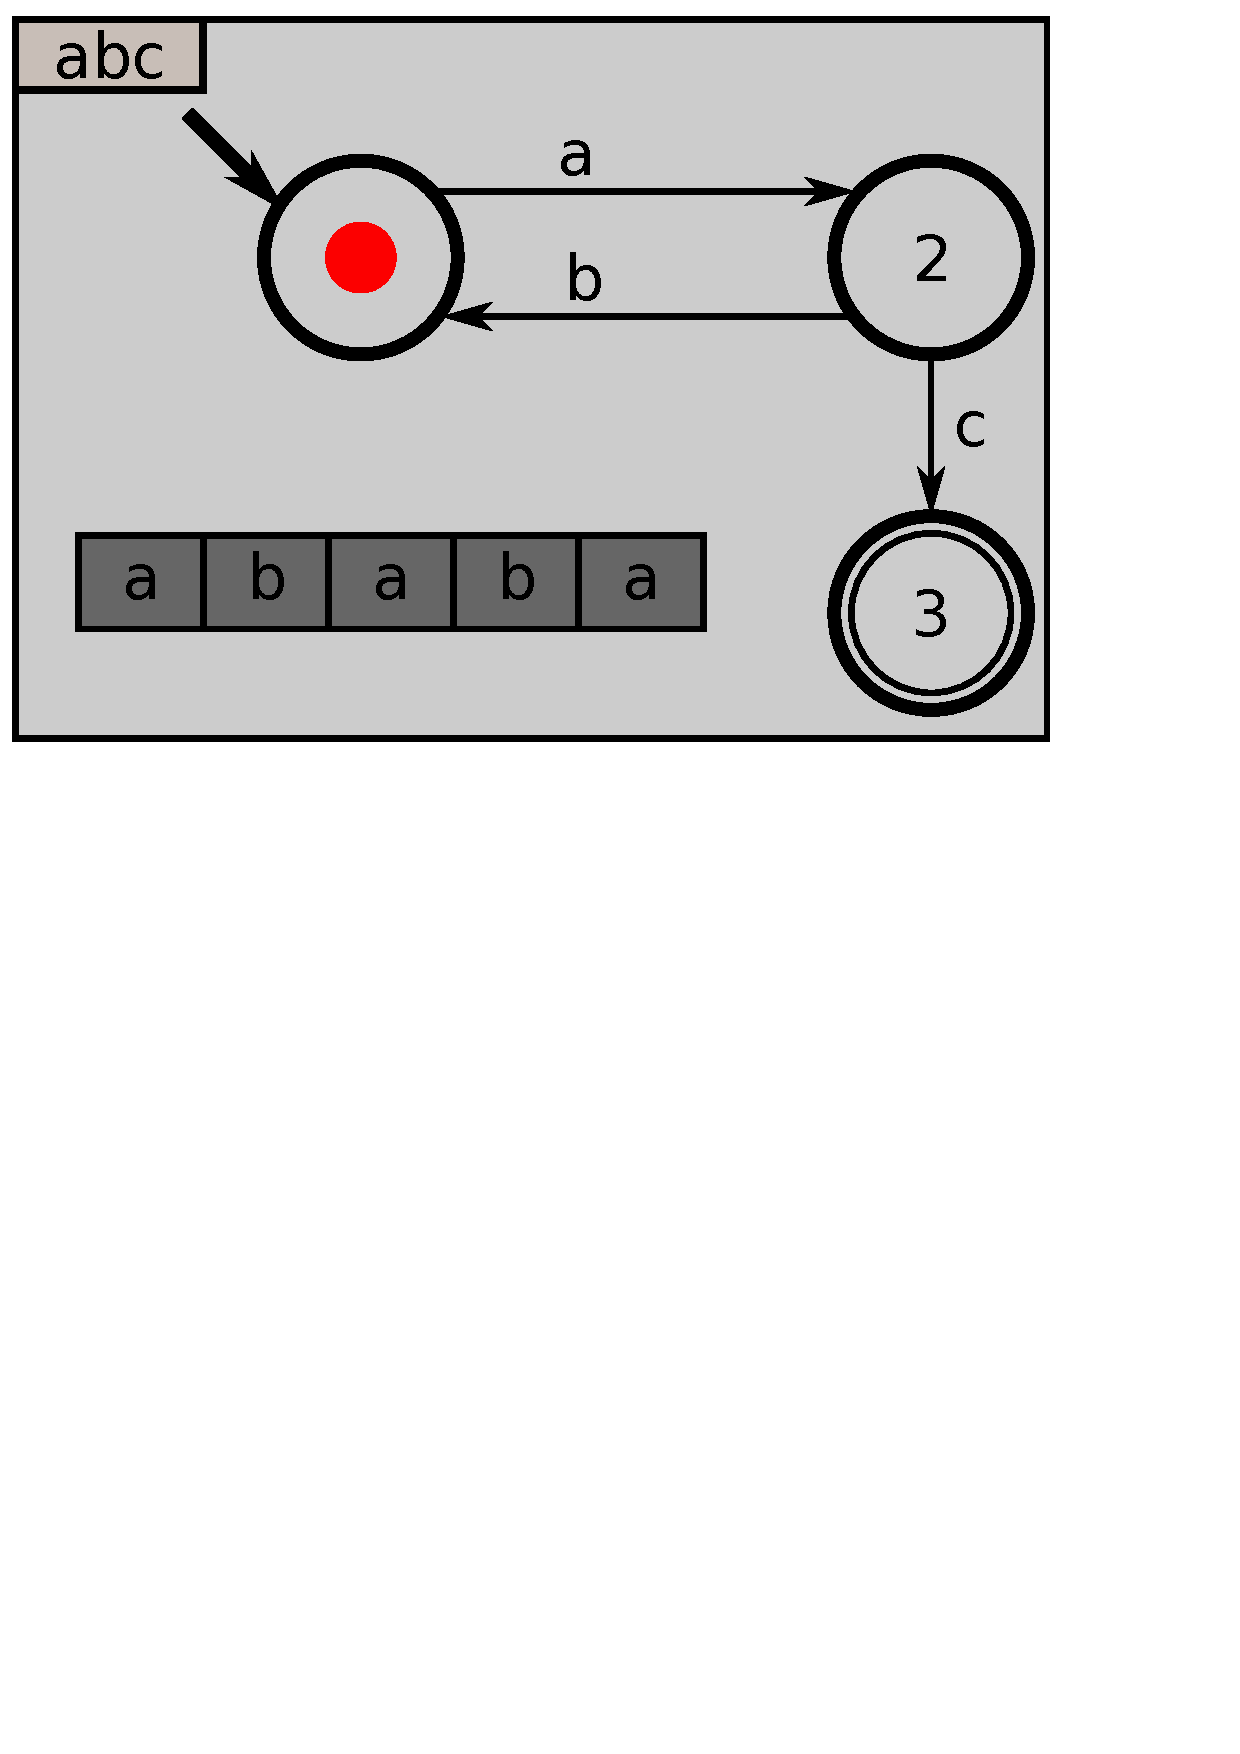
\includegraphics[width=\columnwidth, clip, trim=0cm 17cm 3cm 0cm]{FSM_MX.pdf}%
      \caption{Starting executing \textsf{abc}: the \textsf{current} 
      \textsf{State} is overlayed with a red token, and attempting to accept the
      word \textsf{ababa}.}
      \label{fig:FSM:Model:Execution}
   \end{subfigure}
  
   \vskip\baselineskip
   \begin{subfigure}[b]{0.45\columnwidth}
      \centering
      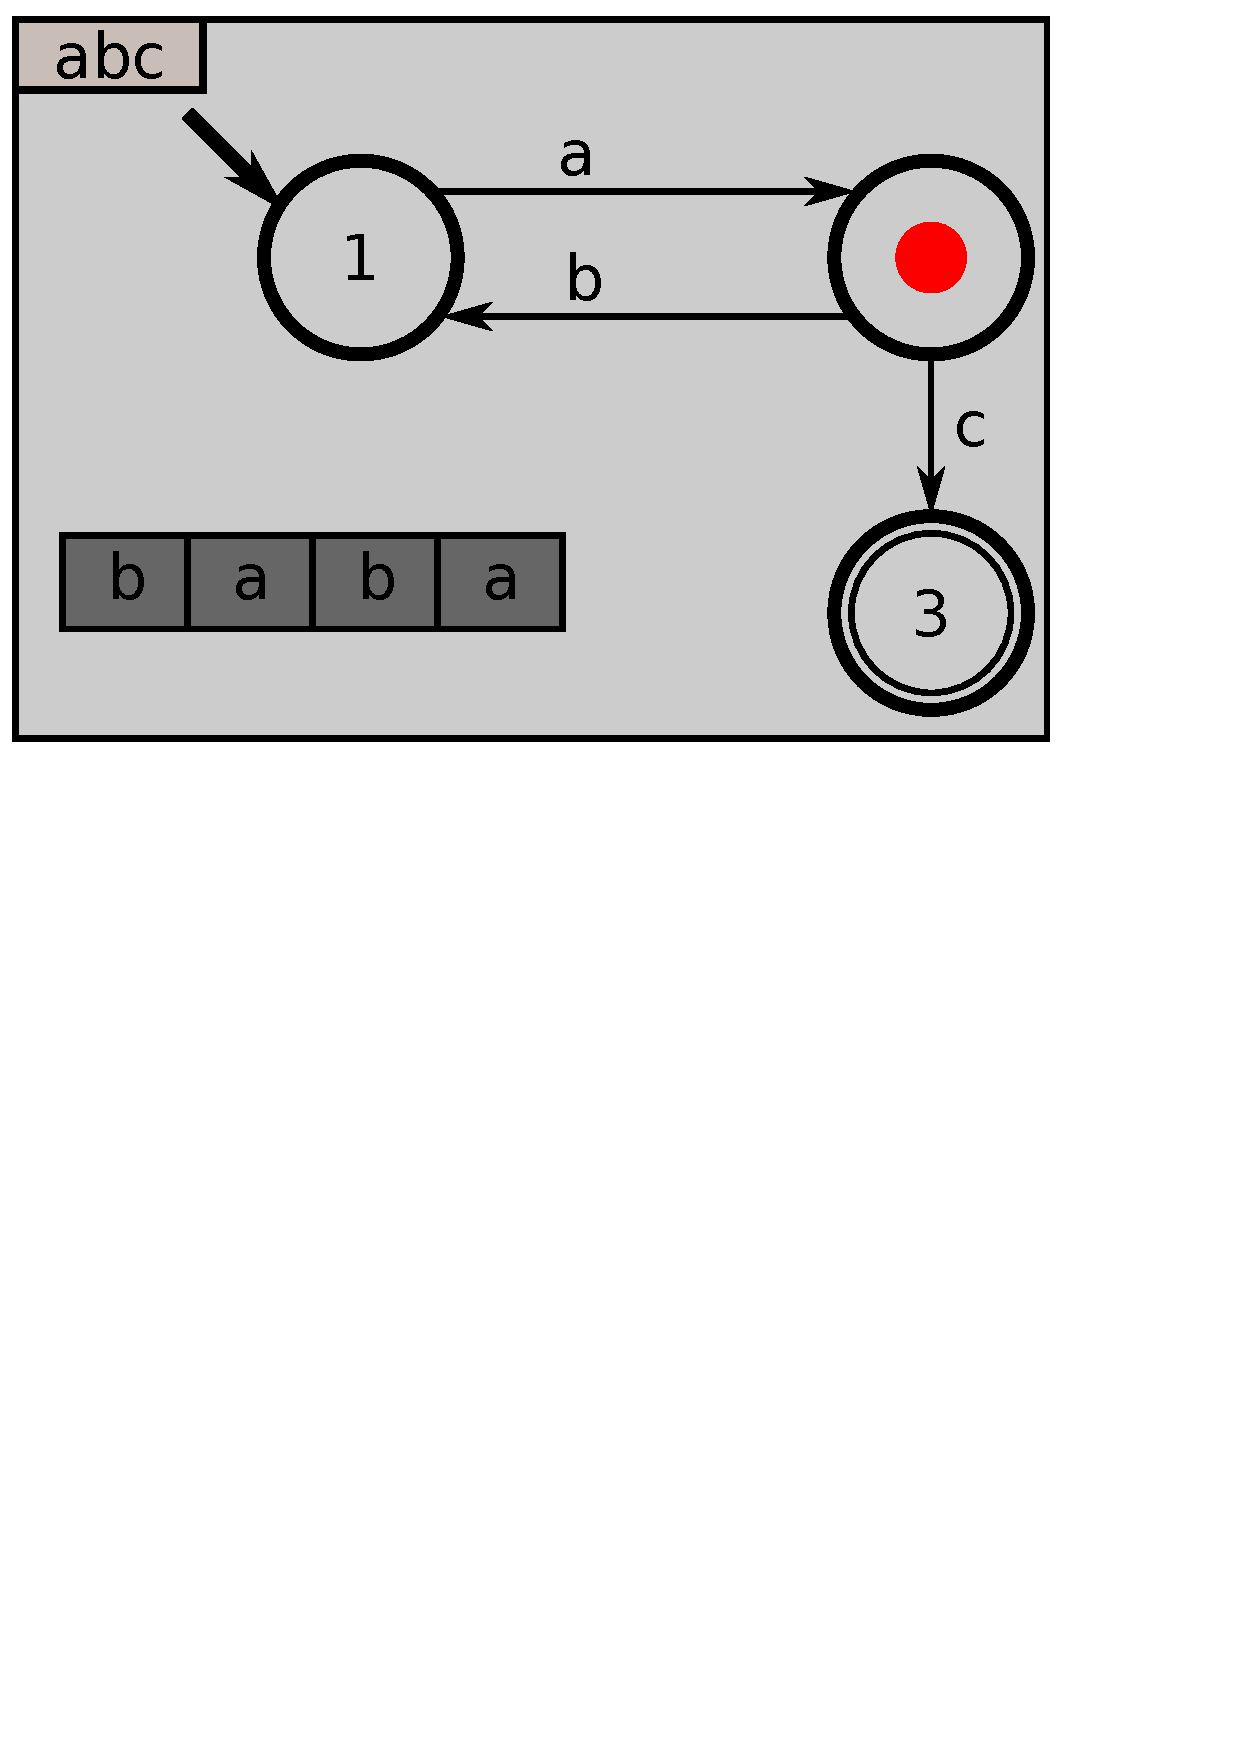
\includegraphics[width=\columnwidth, clip, trim=0cm 17cm 3cm 0cm]{FSM_MA11.pdf}%
      \caption{\textbf{Animation FSM.1:} The first execution step moves the token in
      \textsf{State} 2 (while consuming the first \textsf{Element} \textsf{a}).}
      \label{fig:FSM:Model:Animation:FSA1.1}
   \end{subfigure}
   \hfill
   \begin{subfigure}[b]{0.45\columnwidth}
      \centering
      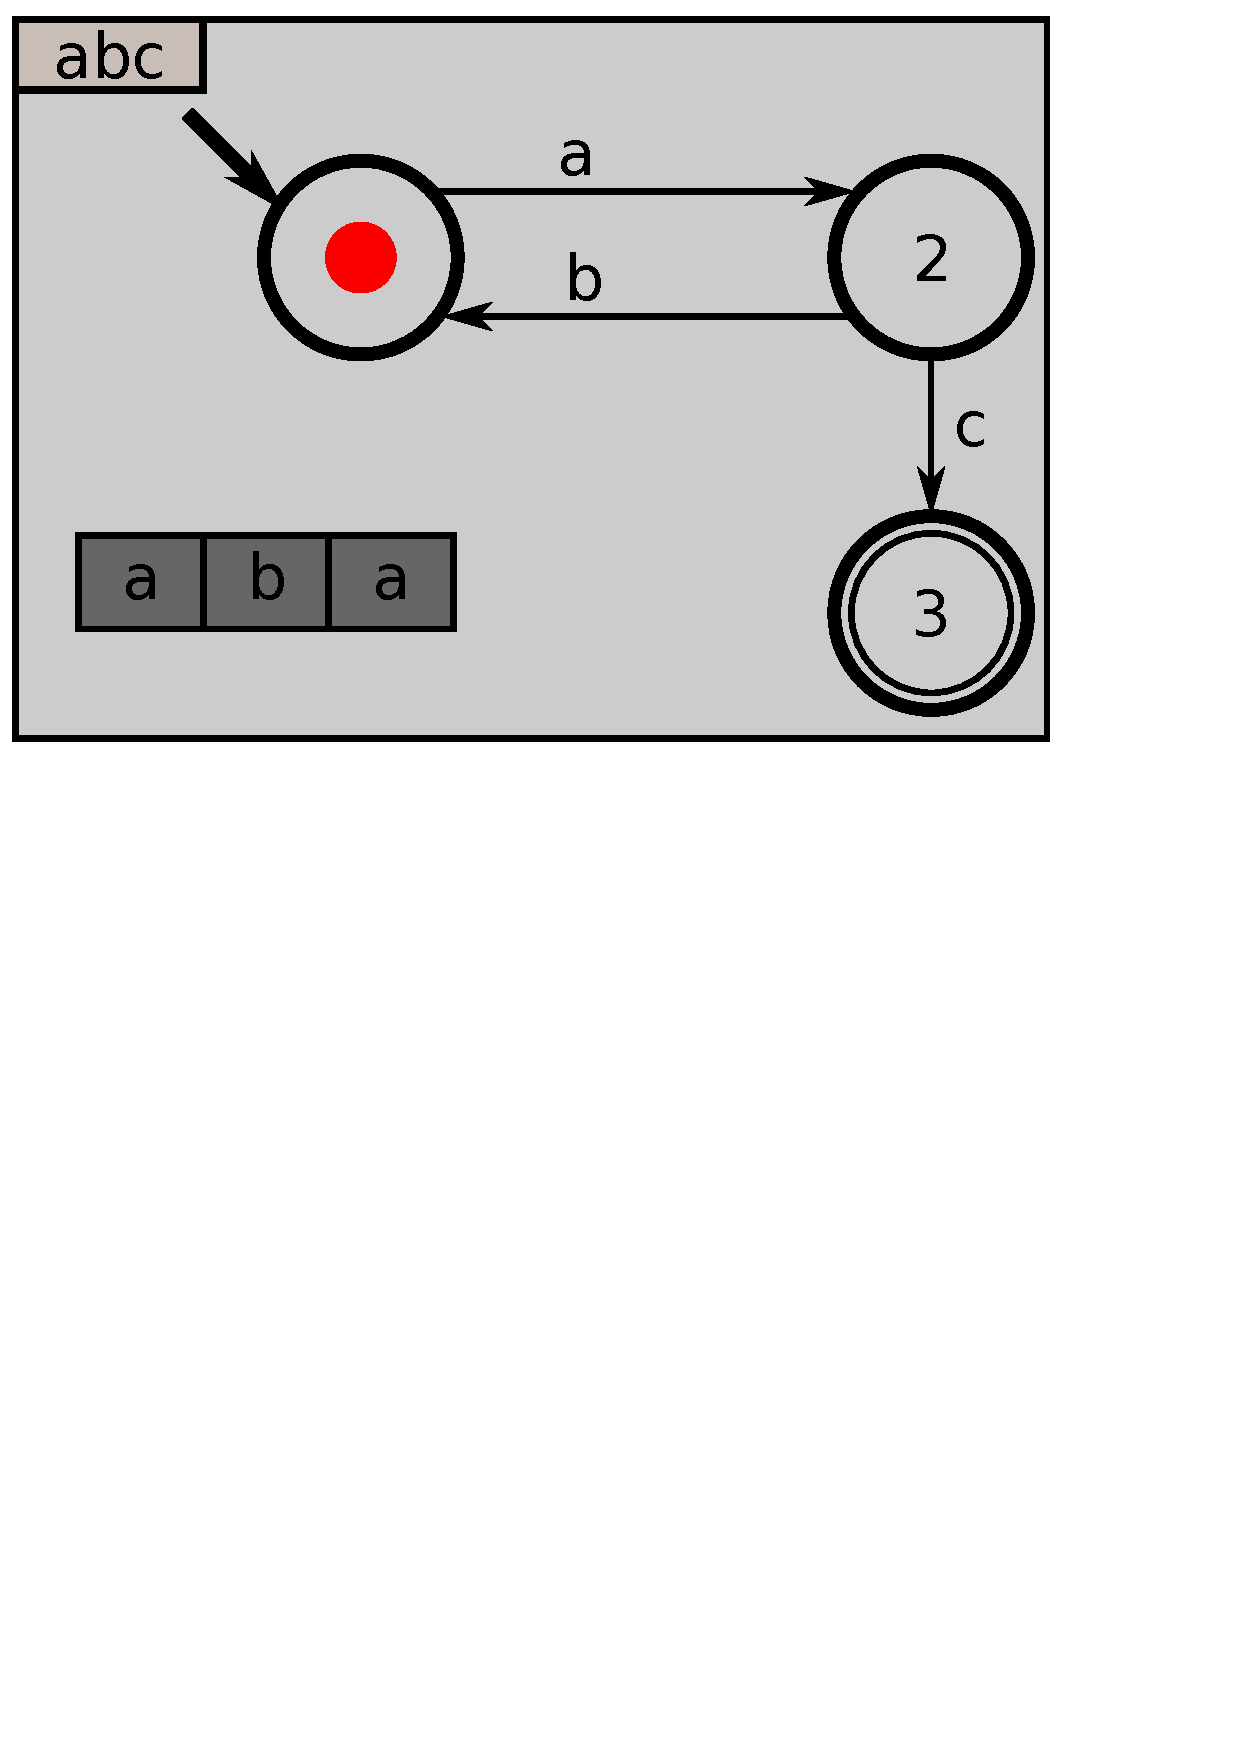
\includegraphics[width=\columnwidth, clip, trim=0cm 17cm 3cm 0cm]{FSM_MA12.pdf}%
      \caption{\textbf{Animation FSM.1:} The second execution step moves the token 
      back in \textsf{State} 1 (while consuming \textsf{b}).}
      \label{fig:FSM:Model:Animation:FSA1.2}
    \end{subfigure}
 
    \vskip\baselineskip
    \begin{subfigure}[t]{0.45\columnwidth}
      \centering
      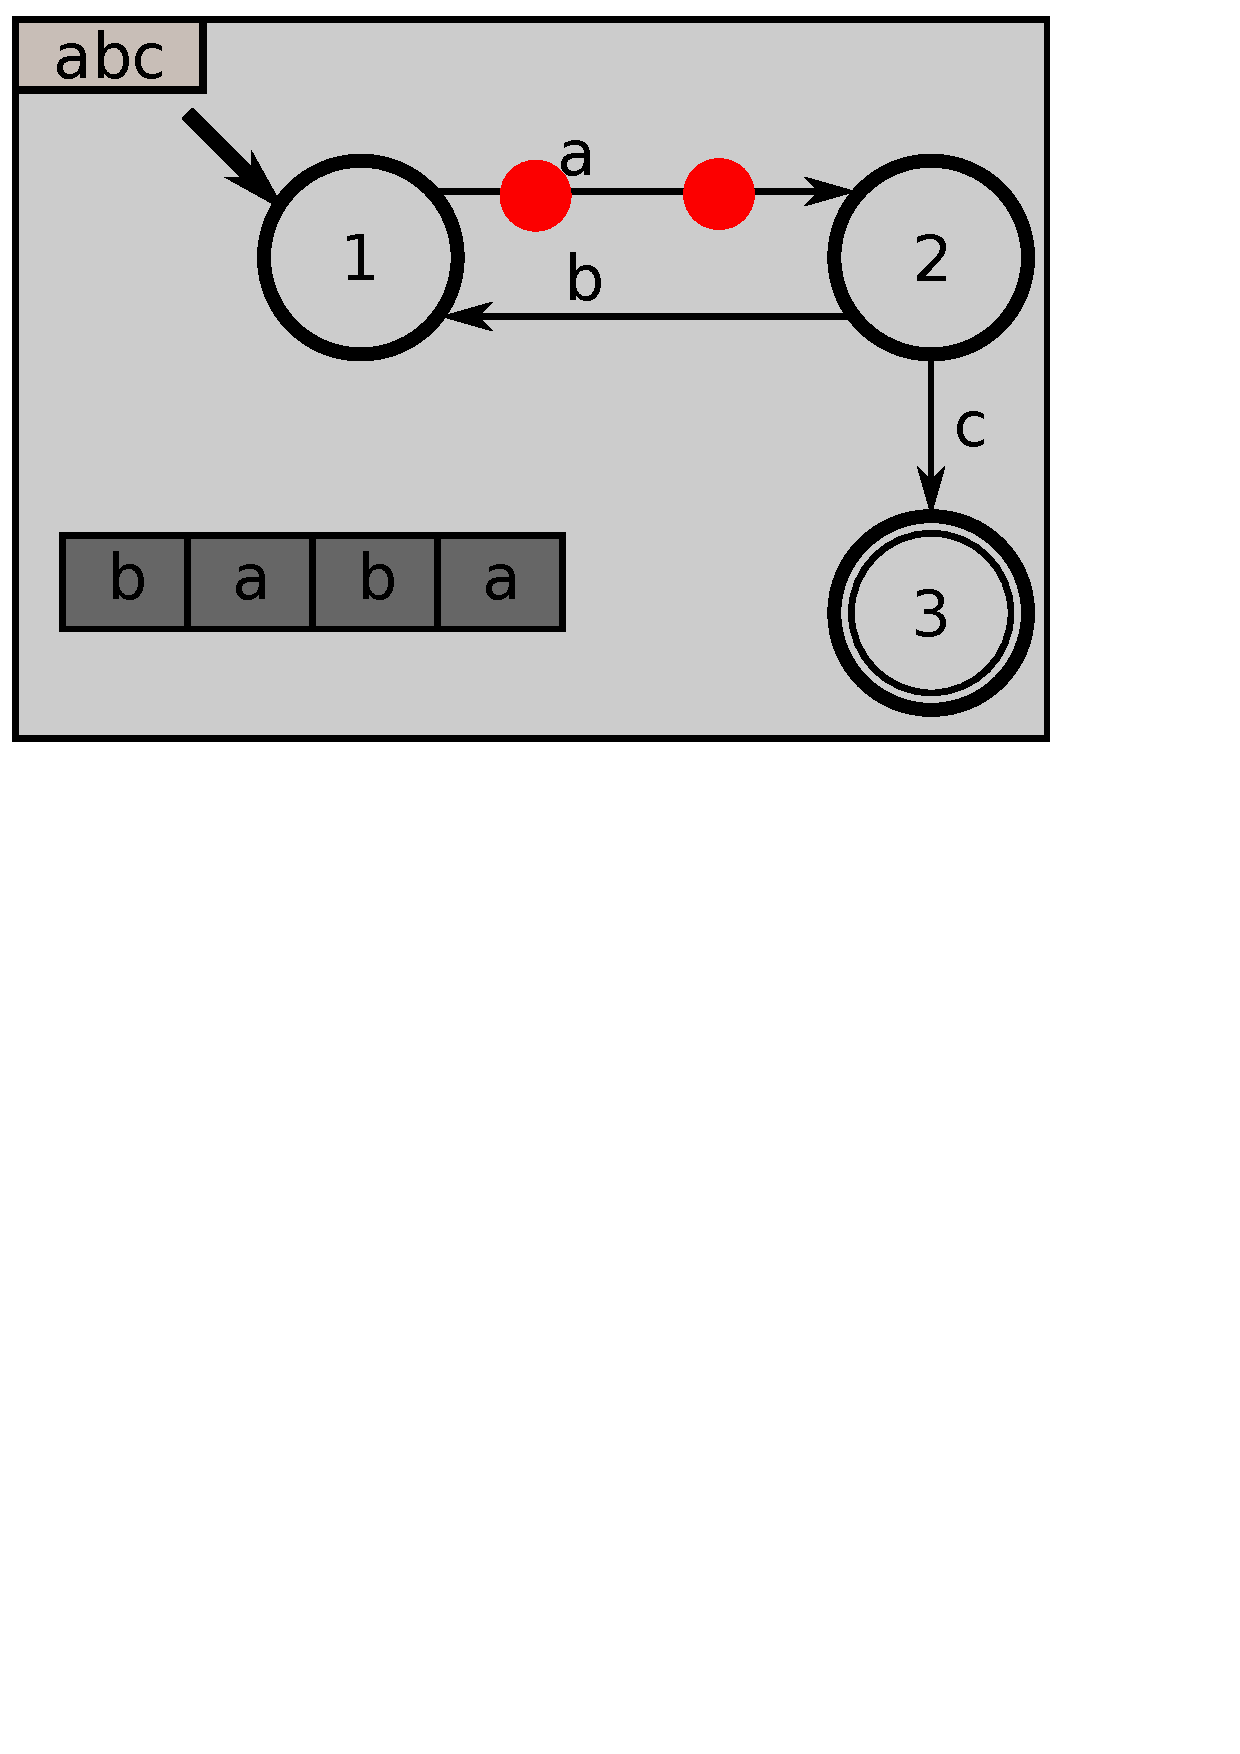
\includegraphics[width=\columnwidth, clip, trim=0cm 17cm 3cm 0cm]{FSM_MA21.pdf}%
      \caption{\textbf{Animation FSM.2:} The first phase of the animation slides
      token along the \textsf{Transition} \textsf{a} (represented here in two 
      different positions to reproduce the animation's visual effect).}
      \label{fig:FSM:Model:Animation:FSA2.1}
    \end{subfigure}
    \hfill
    \begin{subfigure}[t]{0.45\columnwidth}
      \centering
      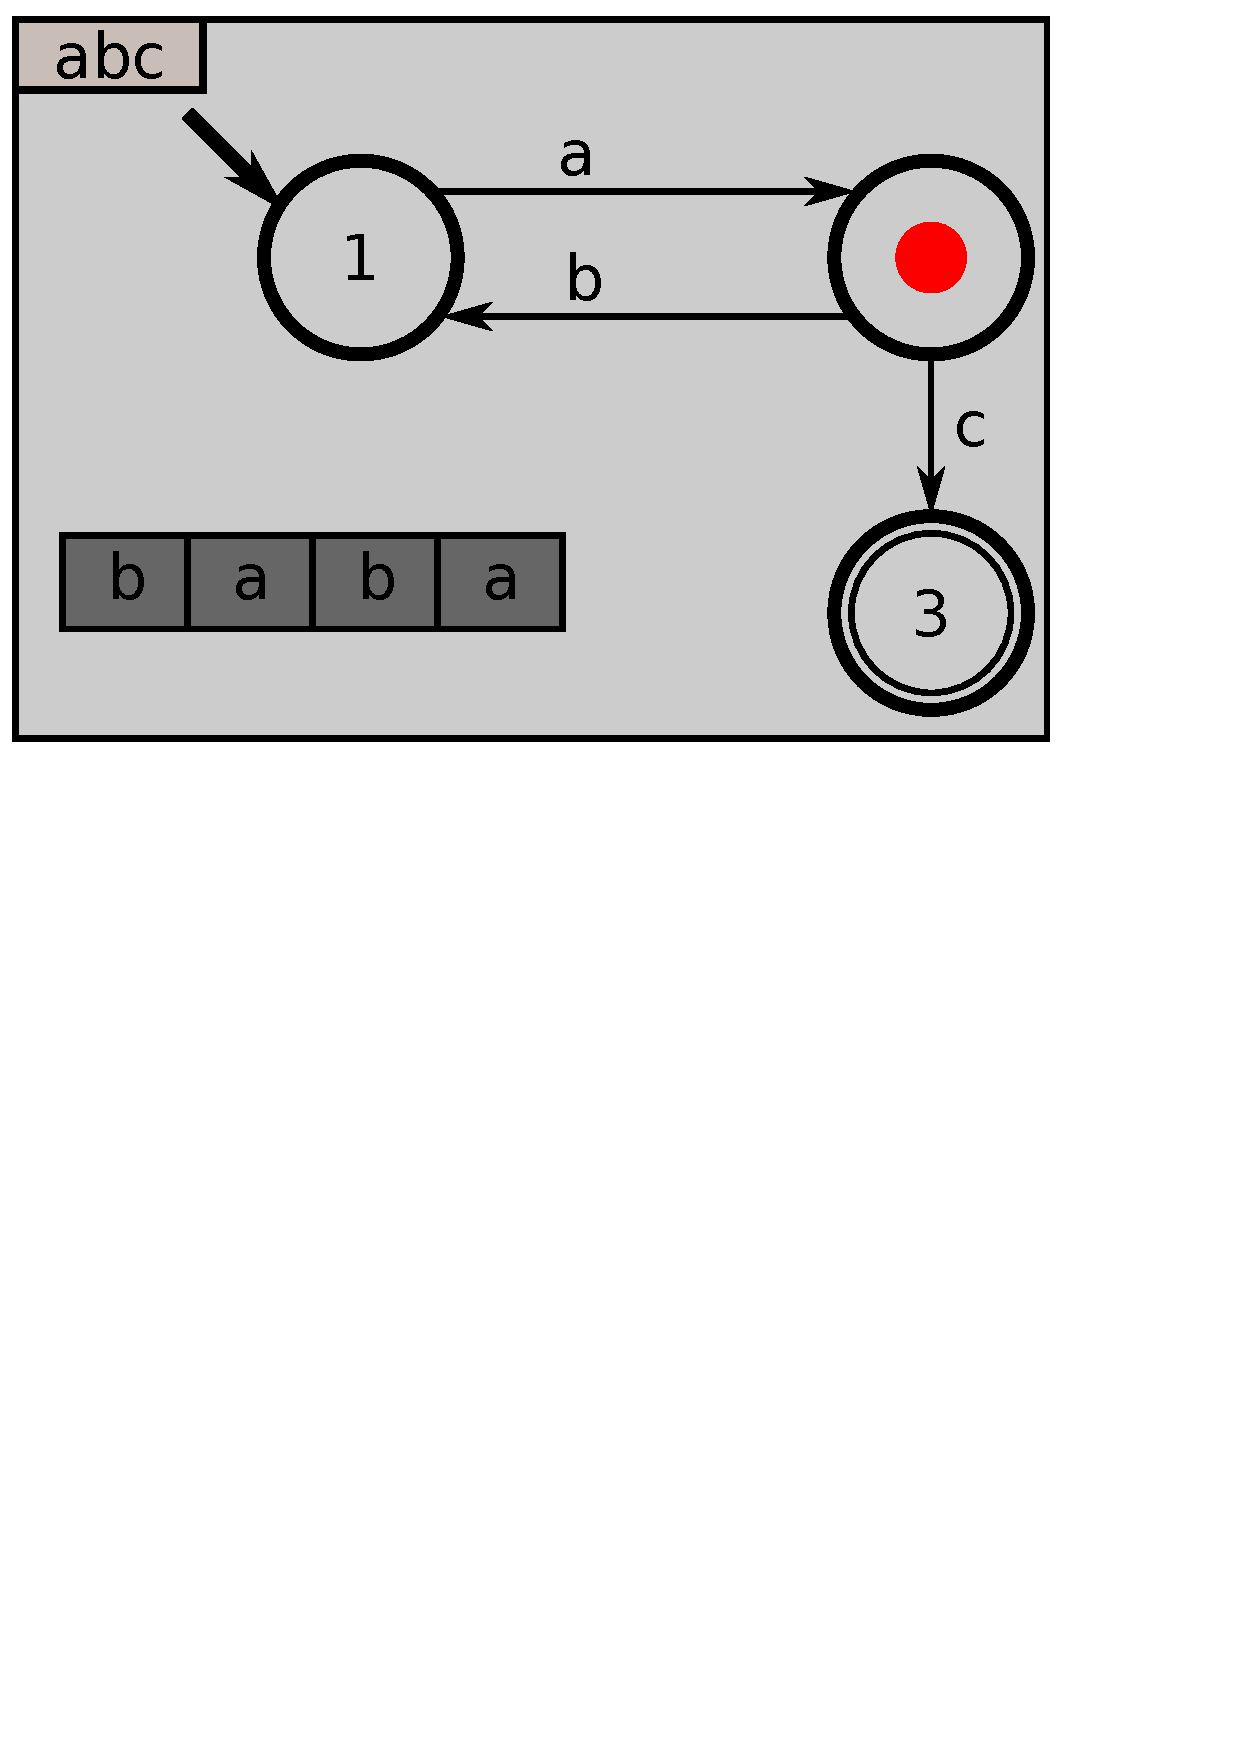
\includegraphics[width=\columnwidth, clip, trim=0cm 17cm 3cm 0cm]{FSM_MA22.pdf}%
      \caption{\textbf{Animation FSM.2:} The second phase of the animation makes
      the token appears in \textsf{State} 2, after consuming \textsf{b}.}
      \label{fig:FSM:Model:Animation:FSA2.2}
    \end{subfigure}

    \vskip\baselineskip
    \begin{subfigure}[t]{0.45\columnwidth}
      \centering
      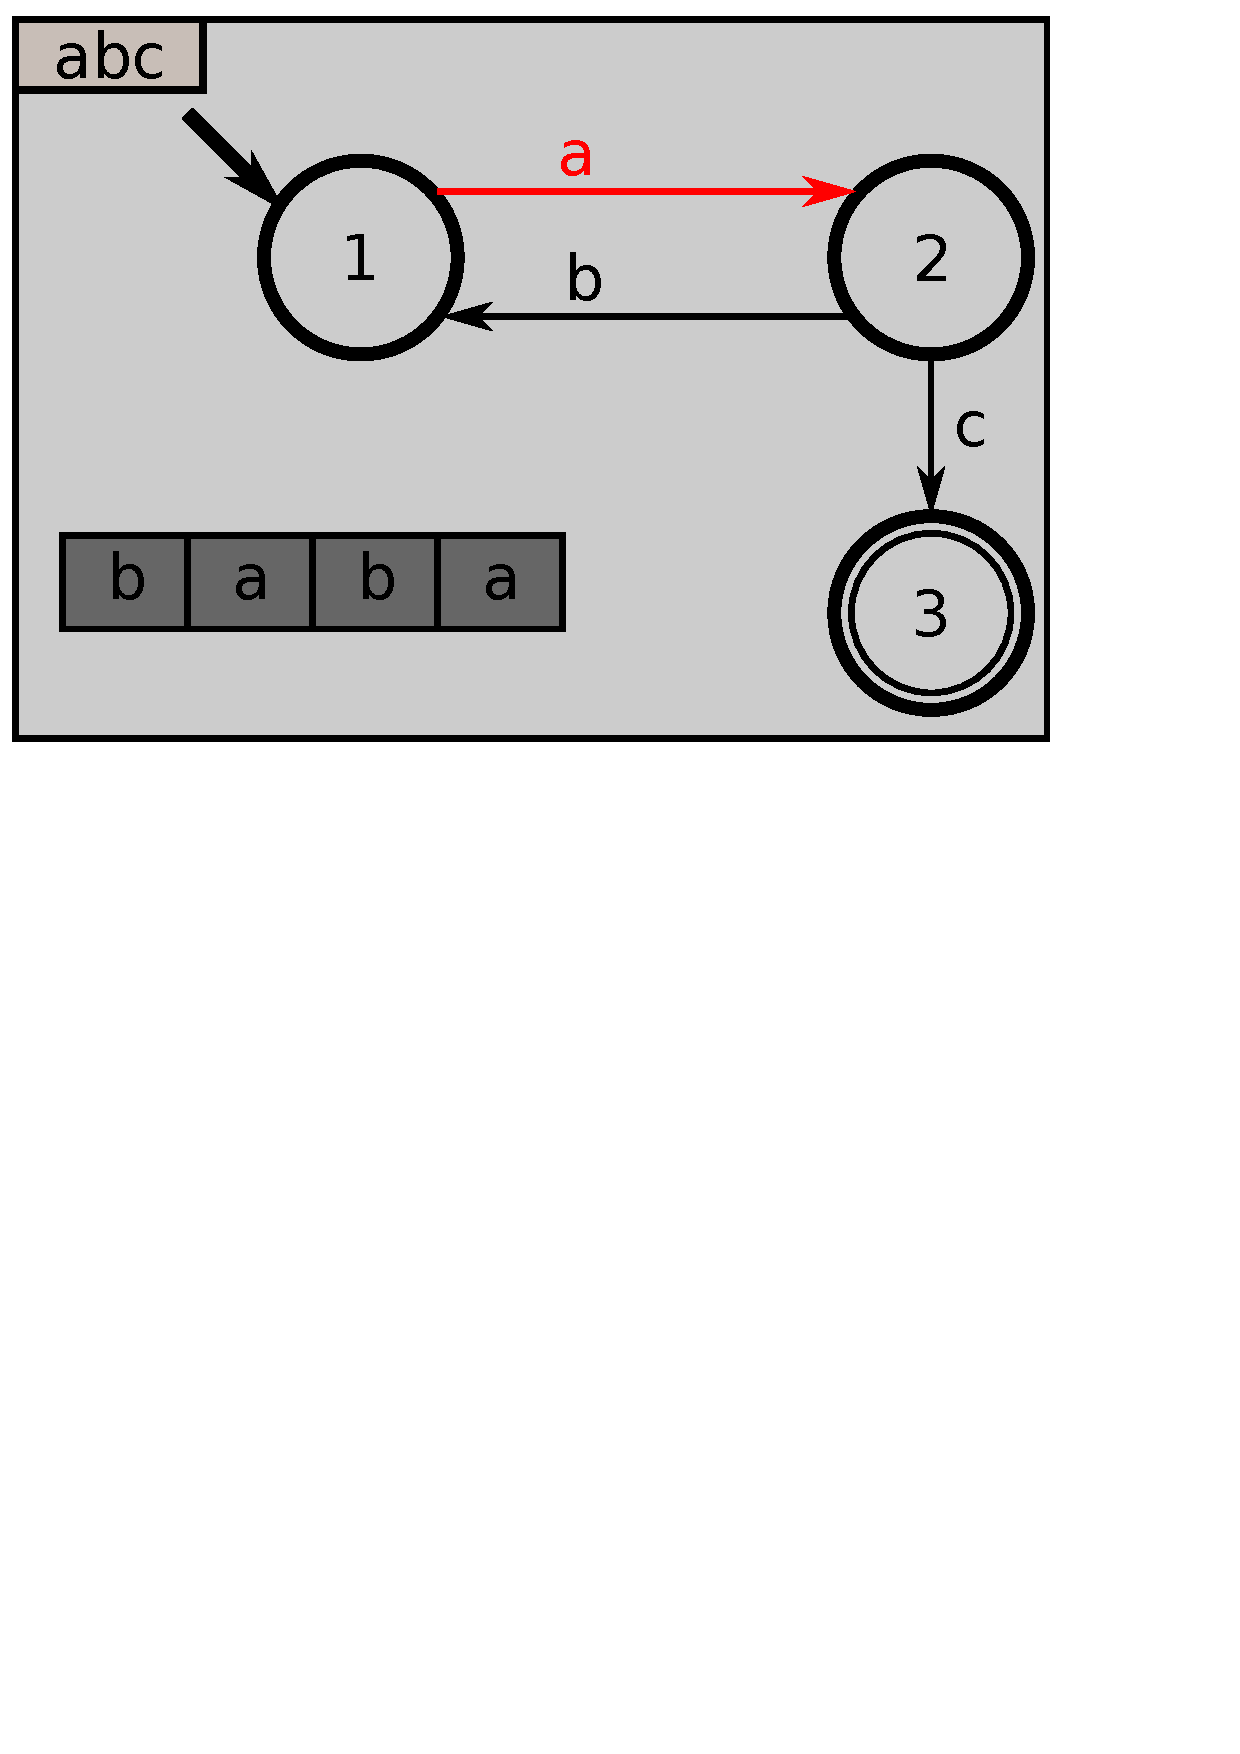
\includegraphics[width=\columnwidth, clip, trim=0cm 17cm 3cm 0cm]{FSM_MA31.pdf}%
      \caption{\textbf{Animation FSM.3:} The first phase of the animation highlights
      \textsf{Transition} \textsf{a} in red (as well as its \textsf{Trigger}).}
      \label{fig:FSM:Model:Animation:FSA2.3}
    \end{subfigure}
    \hfill
    \begin{subfigure}[t]{0.45\columnwidth}
      \centering
      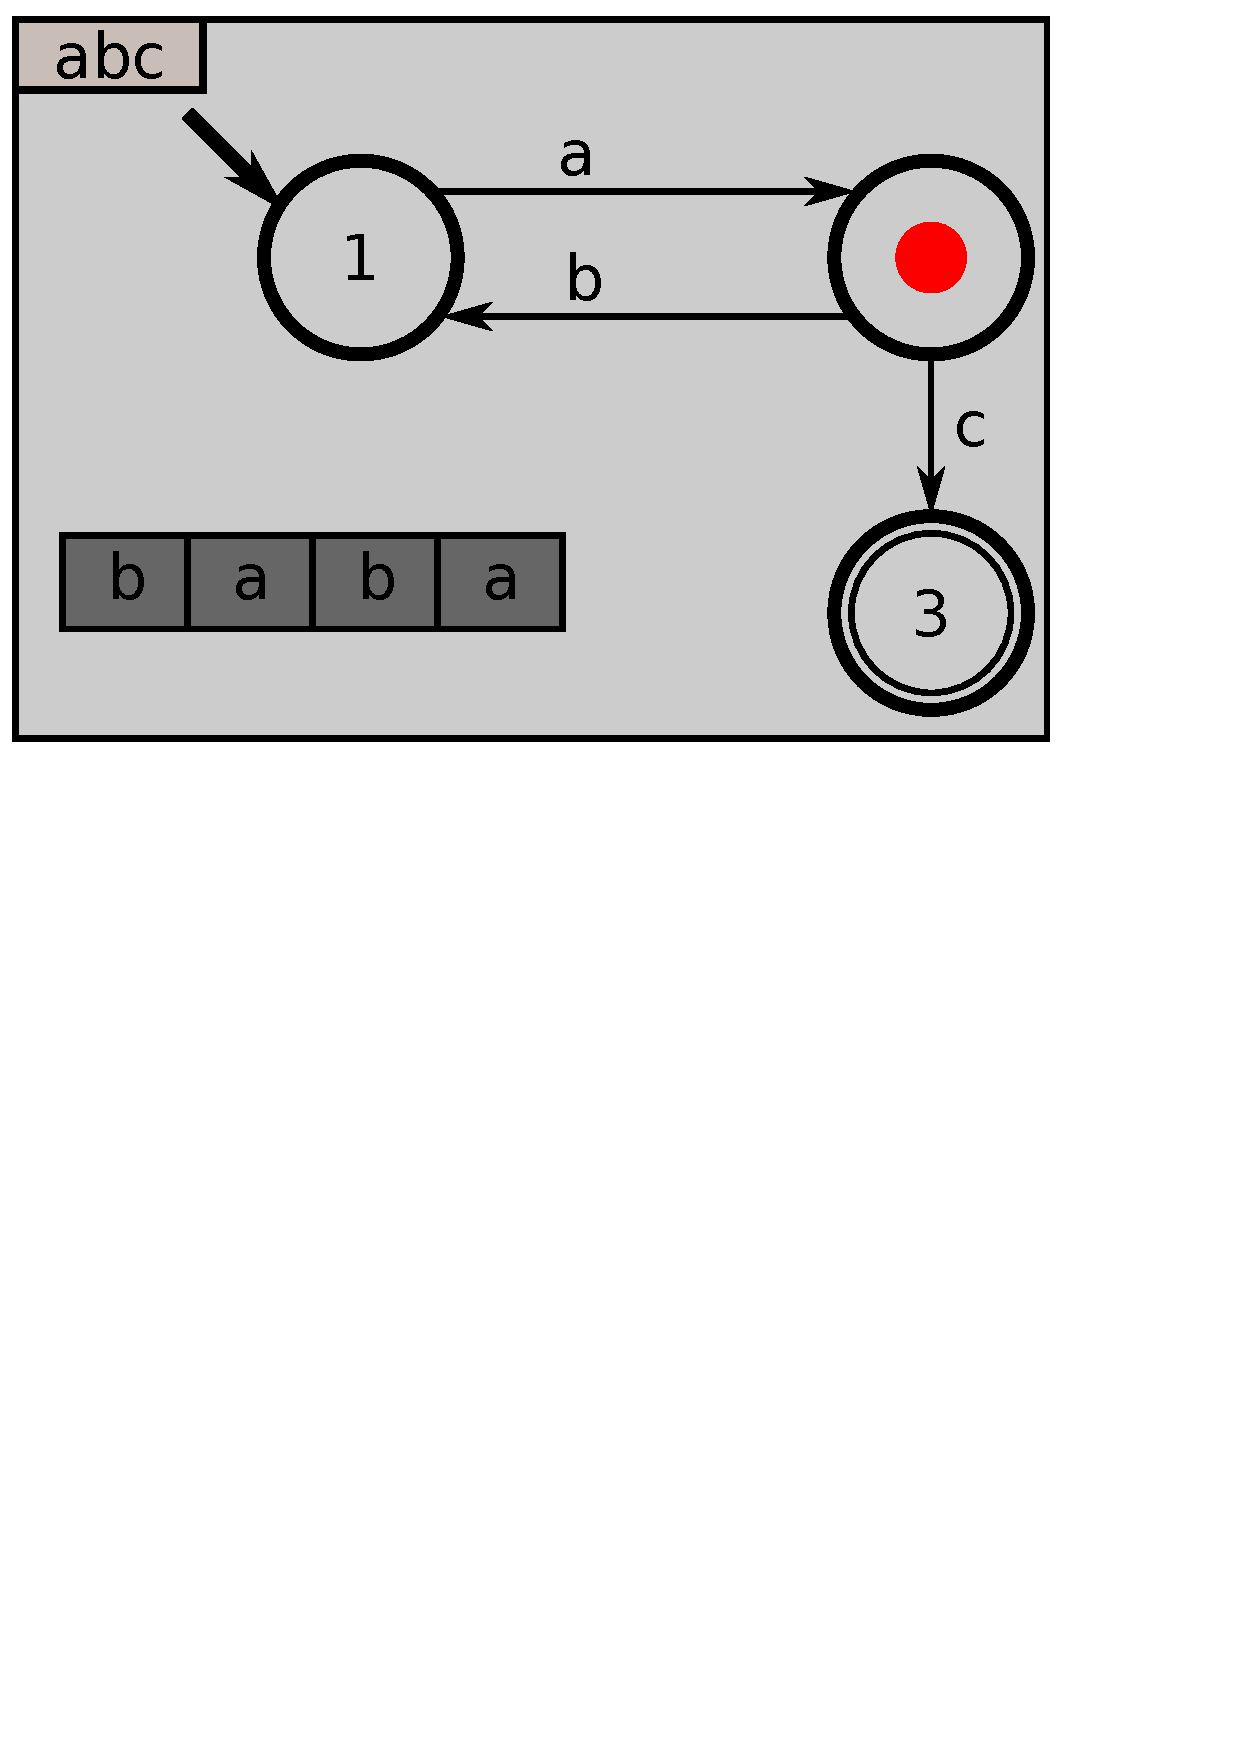
\includegraphics[width=\columnwidth, clip, trim=0cm 17cm 3cm 0cm]{FSM_MA22.pdf}%
      \caption{\textbf{Animation FSM.3:} The second phase of the animation makes
      the token appears in \textsf{State} 2, after consuming \textsf{b}.}
      \label{fig:FSM:Model:Animation:FSA2.4}
    \end{subfigure}

  \caption{\textsf{abc}: a simple model of an FSM conforming to the specification
   in \autoref{fig:FSM_MM}, and some associated animations for its execution 
   (cf. \S \ref{sec:Examples:FSM:Animations} for their specification.)}%
   \label{fig:FSM_M}%
\end{figure}

